\chapter{Cell detection results}
	\label{app:appendix_detectionresults}

\begin{figure}
	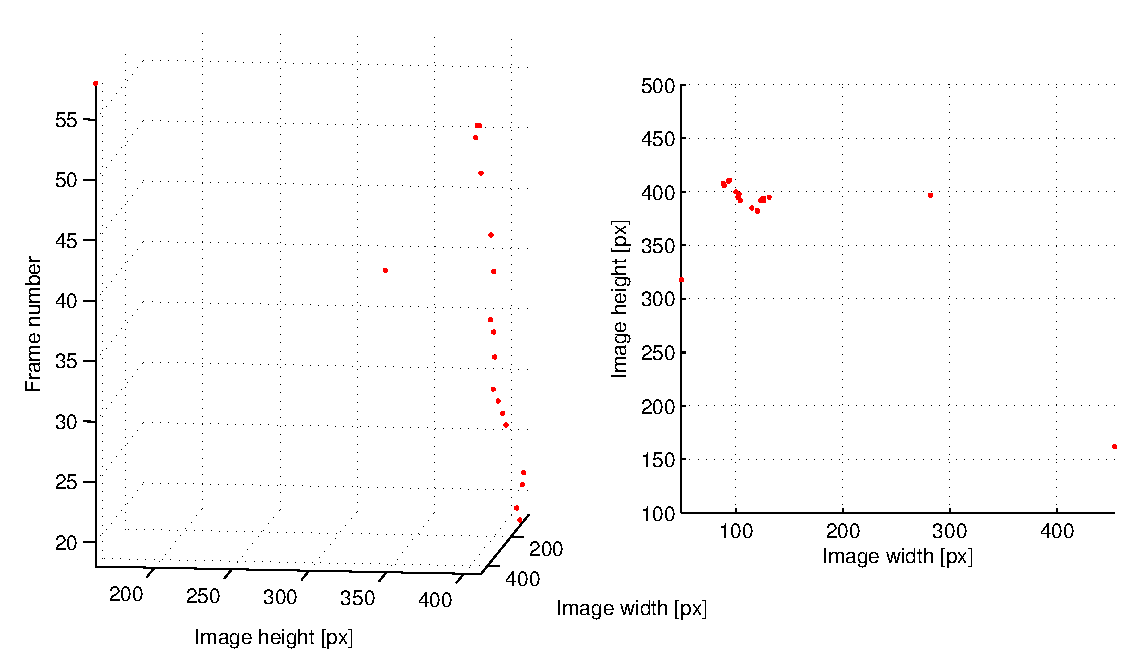
\includegraphics[width=\textwidth]{images/fig_results_detector_sequences_1}
	\caption{Three-dimensional view and orthographic projection from the top of the detection results for dataset A.}
	\label{fig:results_detector_sequences_1}
\end{figure}

\begin{figure}
	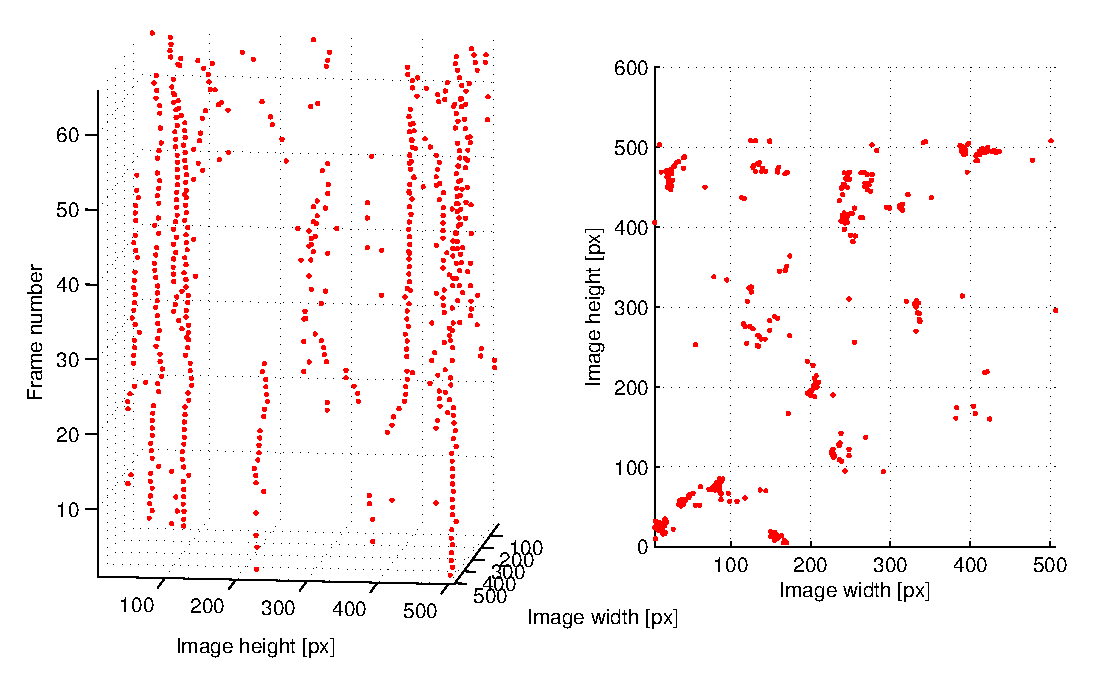
\includegraphics[width=\textwidth]{images/fig_results_detector_sequences_2}
	\caption{Three-dimensional view and orthographic projection from the top of the detection results for dataset B.}
	\label{fig:results_detector_sequences_2}
\end{figure}

\begin{figure}
	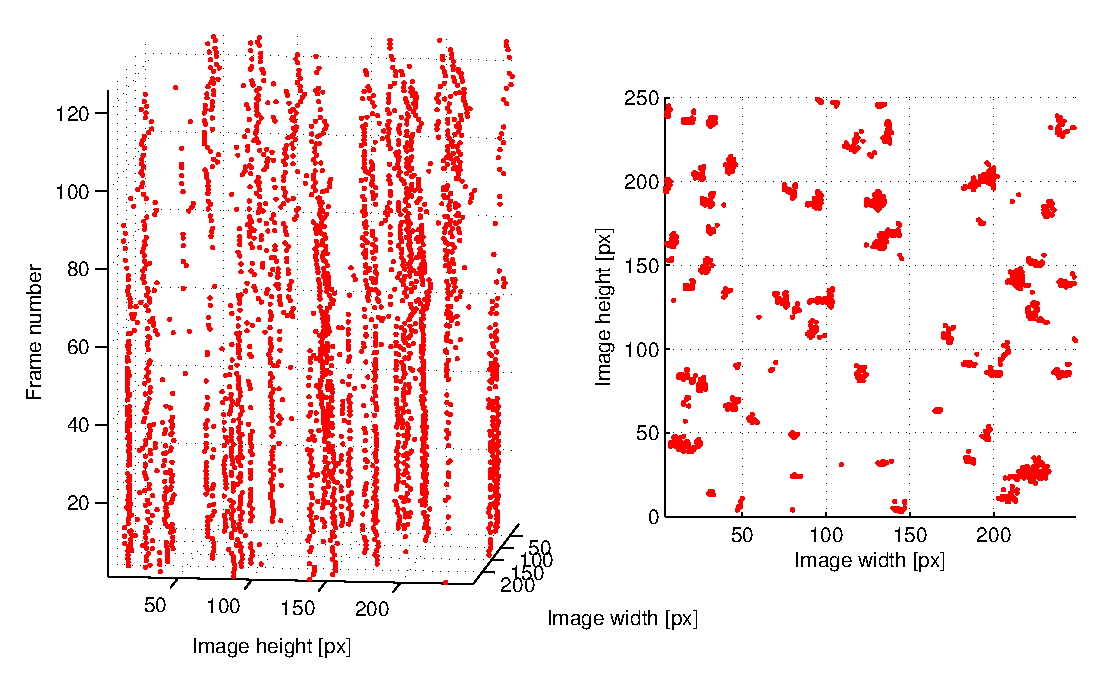
\includegraphics[width=\textwidth]{images/fig_results_detector_sequences_3}
	\caption{Three-dimensional view and orthographic projection from the top of the detection results for dataset C.}
	\label{fig:results_detector_sequences_3}
\end{figure}

\begin{figure}
	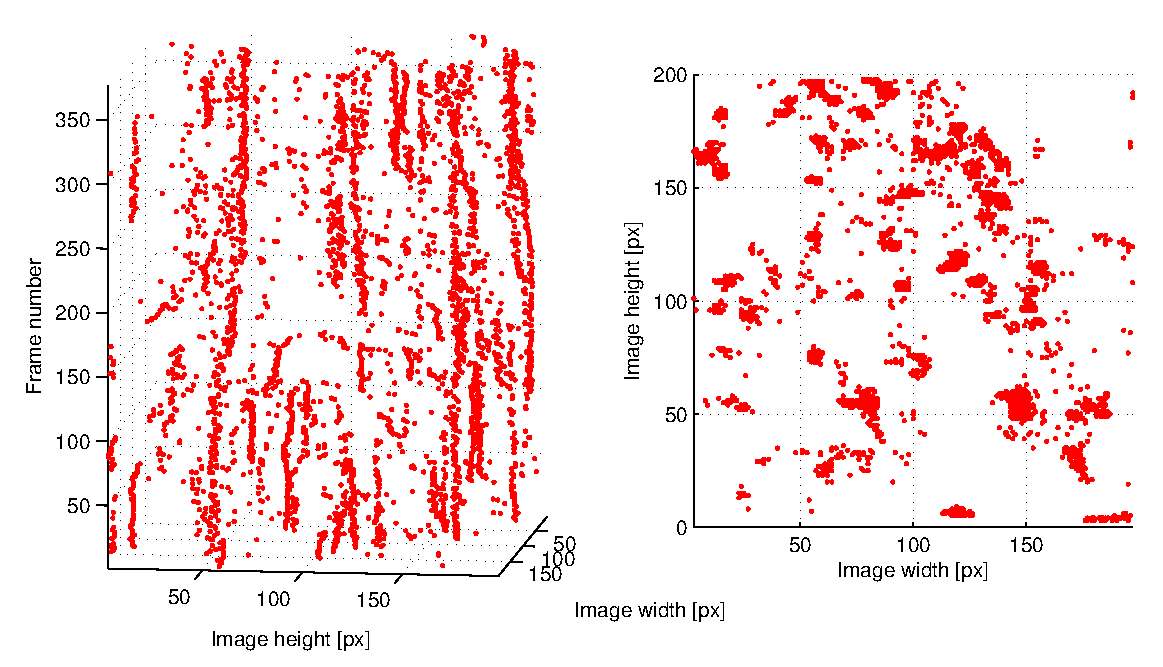
\includegraphics[width=\textwidth]{images/fig_results_detector_sequences_4}
	\caption{Three-dimensional view and orthographic projection from the top of the detection results for dataset D.}
	\label{fig:results_detector_sequences_4}
\end{figure}
\begin{figure}
	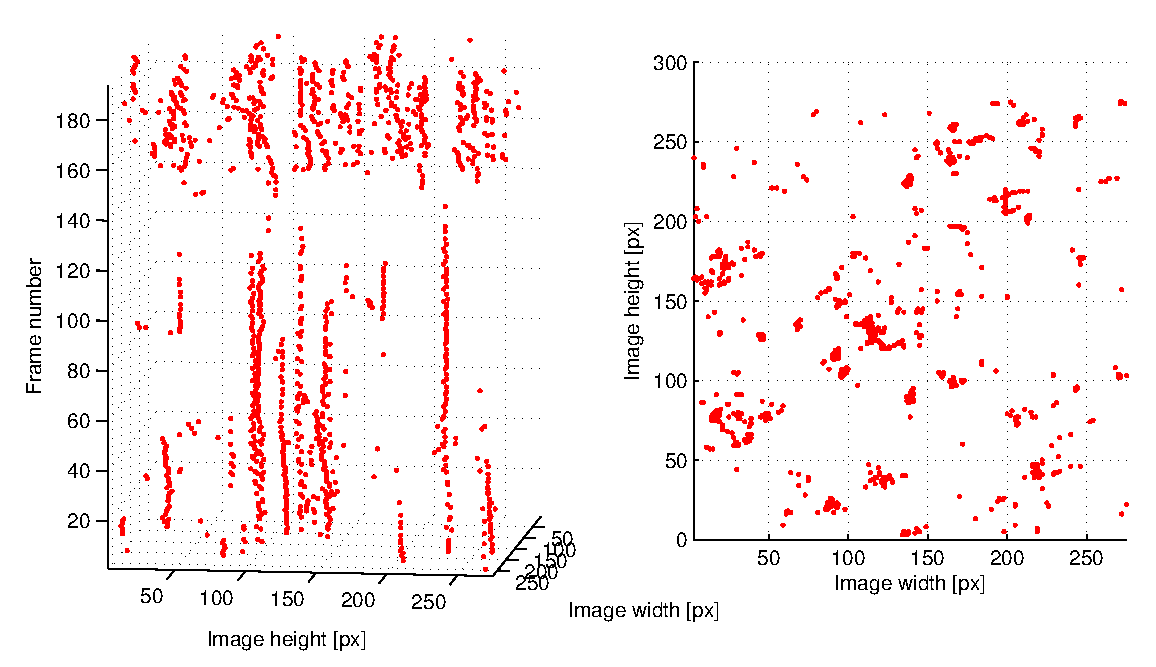
\includegraphics[width=\textwidth]{images/fig_results_detector_sequences_5}
	\caption{Three-dimensional view and orthographic projection from the top of the detection results for dataset E.}
	\label{fig:results_detector_sequences_5}
\end{figure}			